\section{Collaborative ML Workload Optimizations} \label{sec-ml-workloads}
In this section, we provide an overview of of our collaborative ML workload optimization system.
Figure \ref{system-workflow} shows the high-level architecture of our system.
In a typical collaborative environment, users fetch datasets from a central server, perform their analysis on their local machine, and optionally store their results back in the central server.
Our system also comprises of a client and server.
The client is responsible for parsing the user workloads into workload DAGs (Step 1).
The server receives the workload DAGs, using our reuse algorithm finds the optimal execution DAG and sends it back to the client (Step 2).
Finally, the client executes the optimal execution DAG (Step 3) and prompts the materializer to update the Experiment Graph and store the artifacts from the executed workload DAG (Step 4).
%The client supports both python scripts and interactive Jupyter notebooks.
%The client is also responsible for executing a given workload.
%The Experiment Graph resides on the server side, which enables workload optimization through materialization and reuse of ML artifacts.
%After the optimization, the client receives the optimized program and executes it locally.
This architecture enables us to integrate into existing collaborative environment without requiring any changes to the current workflow.
In the rest of this section, we describe the process of parsing, generating workload DAGs, and executing the workloads.
Then, we describe the process of constructing the Experiment Graph and how we utilize the Experiment Graph in our materialization and reuse algorithm. 
Finally, we address the integration process and the impact of our system on the use case in Section \ref{subsec-motivational-example}.

\begin{figure}
\centering
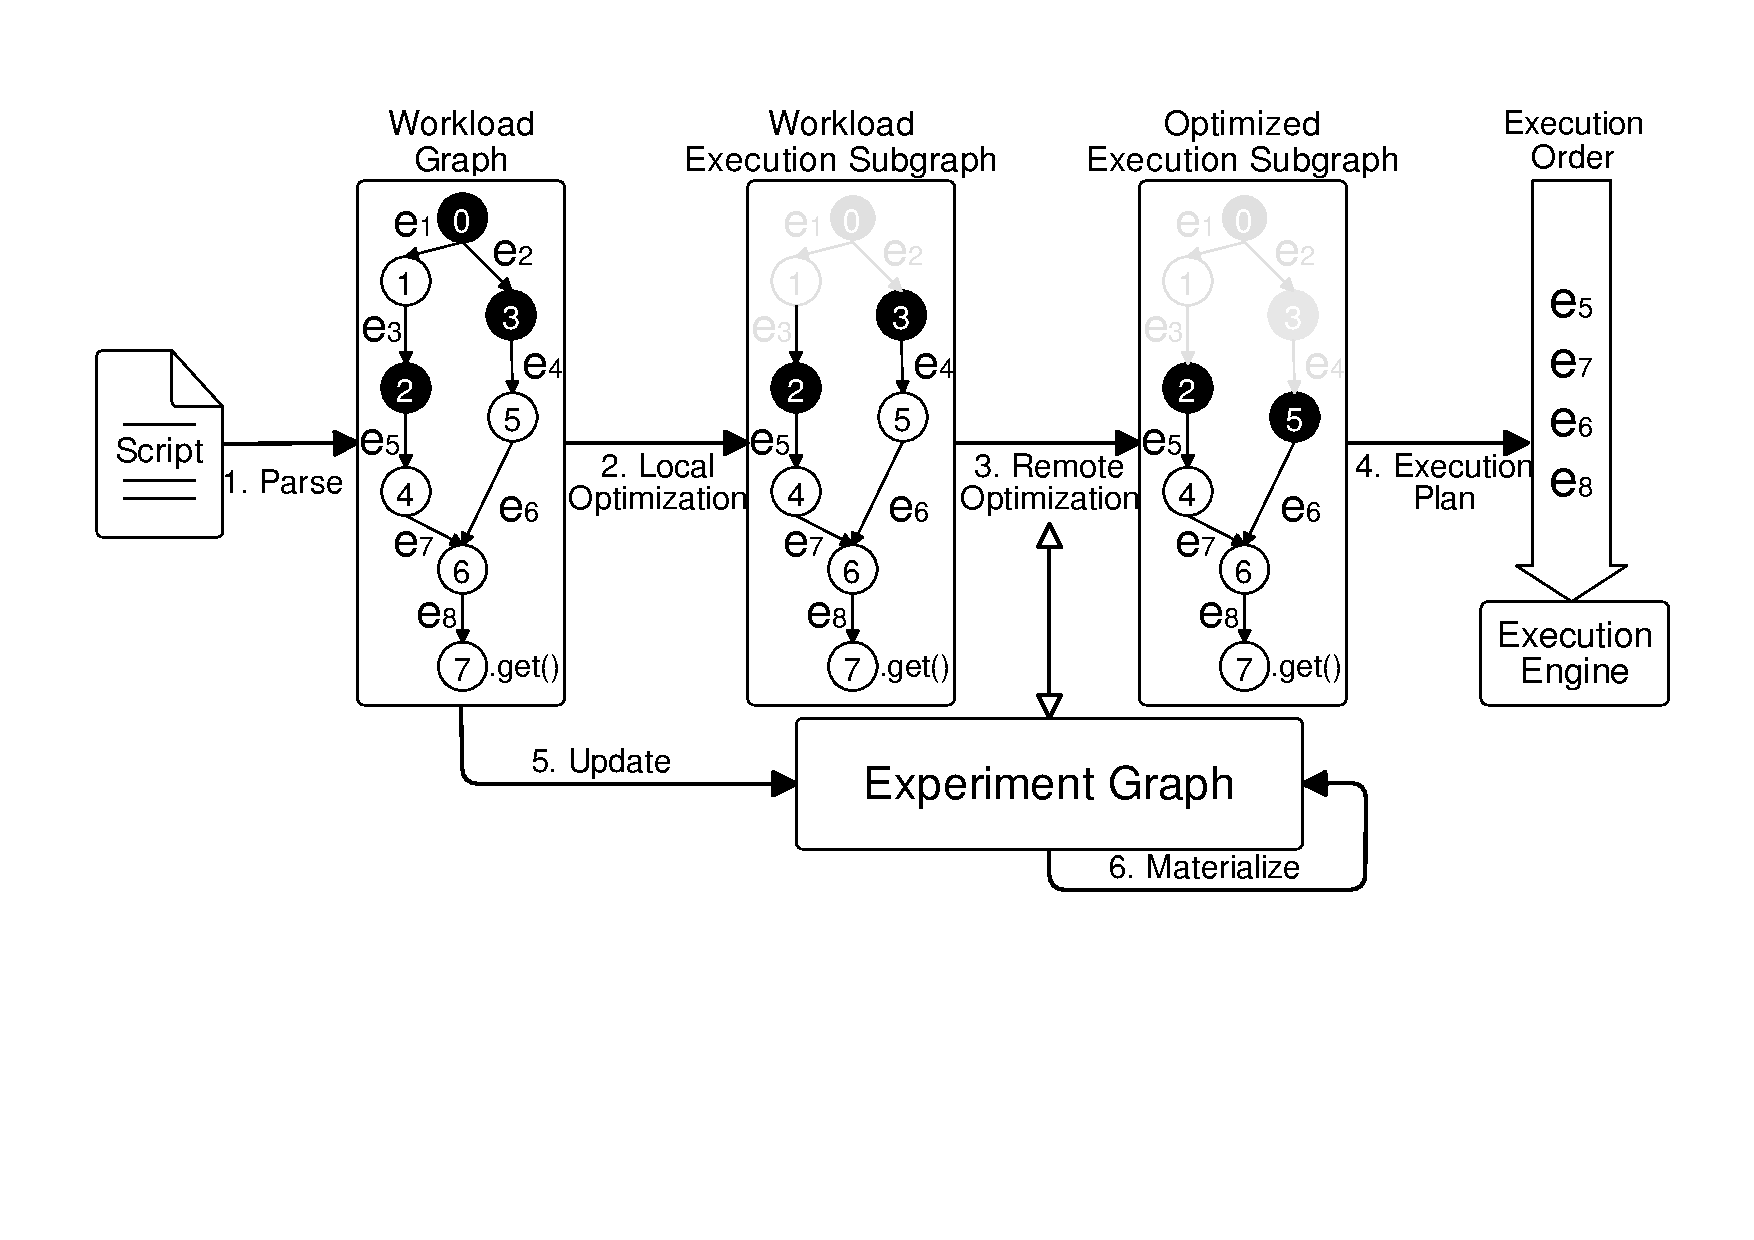
\includegraphics[width=0.7\columnwidth]{../images/system-workflow}
\caption{System overview of the collaborative workload optimizer}
\label{system-workflow}
\end{figure}

\subsection{Client Components}
\textbf{Parser. }
Instead of designing a new DSL, we extend the existing Pandas and scikit-learn \cite{sklearn_api} python packages that are frequently used for data analysis and machine learning workloads.
Upon invocation of the program, the parser transforms the ML workload into a directed acyclic Graph (DAG).
Listing \ref{listing-simple-workload} shows an example of a workload script.
With only a slight modification of the import commands, we are able to load our system's modules.
This enables us to provide support for both python scripts and interactive Jupyter notebooks.
Listing \ref{listing-simple-workload} shows an example of a workload.
\begin{lstlisting}[language=Python, caption=Example script,captionpos=b,label = {listing-simple-workload}]
import custom_pandas as pd

from custom_sklearn import svm
from custom_sklearn.feature_selection import SelectKBest
from custom_sklearn.feature_extraction.text import CountVectorizer

train = pd.read_csv('../input/train.csv') 
print train.columns # [ad_desc,ts,u_id,price,y]
ad_desc = train['ad_desc']
vectorizer = CountVectorizer()
cnt_vect = vectorizer.fit_transform(ad_desc)
selector =  SelectKBest(k=2)
t_subset = train[['ts','u_id','price']]
y =  train['y']
top_feats = selector.fit_transform(
                                  t_subset,  
                                  y )
top_features # print the content of the data frame			     
X = pd.concat([count_vectorized,top_features], axis = 1)
model = svm.SVC().fit(X, train['y'])
print model # terminal vertex
\end{lstlisting}

\textbf{Workload DAG.}
In our DAG representation, vertices represent the artifacts, i.e., raw or preprocessed data (represented by data frame objects) and machine learning models resulting from feature engineering and model training operations and edges represent the operations in the workload.
Each workload DAG has one or more initial vertices representing the raw datasets which are defined as part of the task definition in the collaborative environment.
We refer to these initial vertices as the sources.
A workload DAG also contains one or more terminal vertices.
Terminal vertices represent the output of the workload.
For example, a terminal vertex is a trained ML model, a preprocessed dataset, or an aggregated dataset for visualization. 
Figure \ref{fig-workload-dag} shows an example DAG constructed from the code in Listing \ref{listing-simple-workload}.
\begin{figure}
\centering
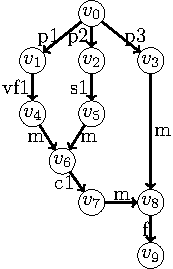
\includegraphics[width=\linewidth]{../images/tikz-standalone/example-graph}
\caption{Workload DAG constructed from the Listing \ref{listing-simple-workload}. The highlighted node shows a terminal vertex.}
\label{fig-workload-dag}
\end{figure}
Once the user requests the result of a terminal vertex, the client first performs a local pruning of the DAG and then sends the DAG to the server for further processing and optimization.
The local pruning step finds the operation (edges) which are not required to execute to compute the terminal vertex.
There are two scenarios where local pruning is beneficial.
First, the local pruning marks all the edges which are not in the path from a source vertex to the terminal vertex.
This is a simple optimization which removes all the operations whose result are not required.
Second, interactive workloads may process a DAG multiple times, after each cell invocation in the Jupyter notebook.
As a result, the result of some vertices is already available.
The local pruning marks all the operations which were previously executed and ensures the executor will not execute them twice.
For example, in Figure \ref{fig-workload-dag}, if $t_subset$ artifact was previously computed, the local pruning step will remove the edge between $train$ and $t_subset$ before sending the DAG to the server.

\textbf{Executor. }
After the server optimizes a workload DAG, the executor receives the optimized DAG to execute the operations and returns the result to the user.
The executor runs the operations in the optimized DAG in their topological order and returns the result back to the user.
After a successful execution, the executor prompts the materialiezr component to update the Experiment Graph and store the computed artifacts.
%
%\begin{figure}\label{DAG-workflow}
%\begin{subfigure}{\columnwidth}
%\centering
%\includegraphics[width=0.8\linewidth]{../images/tikz-standalone/system-workflow-legend}
%\end{subfigure}
%\begin{subfigure}{0.3\columnwidth}
%\centering
%\includegraphics[width=0.8\linewidth]{../images/tikz-standalone/system-workflow-1}
%\parbox{3cm}{\caption{Original DAG}}
%\end{subfigure}%
%\begin{subfigure}{0.3\columnwidth}
%\centering
%\includegraphics[width=0.8\linewidth]{../images/tikz-standalone/system-workflow-2}
%\parbox{3cm}{\caption{Pruned DAG}}
%\end{subfigure}%
%\begin{subfigure}{0.3\columnwidth}
%\centering
%\includegraphics[width=0.8\linewidth]{../images/tikz-standalone/system-workflow-3}
%\parbox{3cm}{\caption{Optimized DAG}}
%\end{subfigure}
%\label{fig-experiment-graph}
%\caption{Different stages of a Workload DAG. Loaded: an artifact with its underlying data available, Computed: an artifact who is previously computed in an interactive workload, Materialized: an artifact which is available in the Experiment Graph, Null: an artifact which is not yet computed}
%\end{figure}

\subsection{Server Components}
\textbf{Experiment Graph.}
The union of all the workloads DAGs of the previously executed ML workloads forms another DAG, which we refer to as the \textit{Experiment Graph}.
Every vertex in the Experiment Graph has the attributes $frequency$, $size$, and $compute_time$, representing the number of different workloads an artifact appeared in, the storage size of the artifact, and time required to compute the artifact given its input artifacts, respectively.

Every vertex in the Experiment Graph carries the meta-data of the artifact it represent.
If the artifact is a \textit{Dataset}, then its meta-data includes the name, type, and total size of each column of the data.
If the artifact is a \textit{Model}, its meta-data includes the name, type, hyperparameters, and the error metric of the model.
The decision to store the underlying content of an artifact, i.e., Pandas dataframe and model weights, is left to the materializer component.

The Experiment Graph maintains the list of all the source vertices that it contains.
Furthermore, every edge in the graph stores the hash of the operation it represents.
Therefore, given a workload DAG, the Experiment Graph can quickly detect if it contains any of the artifacts of the workloa DAG.

\textbf{Optimizer. }
The optimizer component is responsible for finding the optimal DAG which incurs the lowest cost when executed.
The optimizer receives the (pruned) workload DAG from the client and for every vertex in the workload DAG, the optimizer queries the Experiment Graph.
The optimizer finds the set of materialized artifacts from the Experiment Graph.
Then, using our reuse algorithm, the optimizer decides what materialized artifacts it should load into the optimized DAG and what artifacts should be recomputed.
The optimizer guarantees the DAG incurs the lowest execution cost, i.e., sum of loading the materialized artifacts and executing the remaining operations.

\textbf{Materializer.}
After the executor finishes the execution of a workload DAG, it annotates the DAG with the execution time and artifact sizes.
The Materializer utilizes this information to decide what artifacts have a high likelihood of reappearing in future workloads.
The Materializer then stores these artifacts in the Experiment Graph.

%Each edge contains the meta-data of the operation it represents, such as the function name, training algorithm, and hyperparameters.
%To uniquely identify an edge, we utilize a hash function which receives as input the operation and its hyperparameters (if it has any).
%Since the experiment graph is rooted, we assign a hash value to every vertex which is computed in the following way:
%\[
%    h(v)= 
%\begin{cases}
%    id,& \text{if } v \text{ is root}\\
%    h\Big(\sum\limits_{e \in in\_edge(v)} (h(e.source) + h(e) ) \Big)  ,              & \text{otherwise}.
%\end{cases}
%\]
%where $in\_edge(v)$ returns the edges with destination $v$. 
%Intuitively, the hash of a root vertex is its unique identifier (location on disk or download URL) and the hashes of other vertices are derived recursively by combining the hashes of their parents and edges which connect them to their parents.

%After a machine learning workload is executed, we update the experiment graph by adding the new artifacts and operations.
%If any of the artifacts already exist in the graph, their frequency is updated.
%We start with an empty Experiment Graph.
%After the execution of the script and updating the Experiment Graph, all the artifacts (vertices) have a frequency of 1.
%To represent operations which process multiple input artifacts, e.g., concat and svm.fit operations in Listing \ref{listing-experiment-graph}, we proceed as follows.
%First, we merge the vertices representing the artifacts into a single vertex using a merge operator.
%The merge operator is a logical operator which does not incur a cost, i.e., it has a run-time of 0 seconds.
%The merged vertex is also a logical vertex with no actual attributes which only contains the vertex ids of the merged vertices.
%Then, we draw an edge from the merged vertex which represents the actual operation.
%For example, in Figure \ref{fig-experiment-graph}a, before applying the concatenation operation, we merge $v_4$ and $v_5$ into $v_6$, then we apply the concatenation operation (c1).
%Furthermore, when computing the hash of a merged vertex, we take the merge order into account.
%For example, the operation svm.fit has $X$ (represented by $v_7$) as first argument and train['y'] (represented by $v_3$) as its second argument.
%When computing hash of $v_8$, we combine the parents in the same order, i.e., $h(v_8) = h(h(v_7) + m + h(v_3) + m)$. 
%After the DAG is constructed, its execution is invoked with the call to the $get()$ command on Line 18.
%\subsection{System Architecture and Workflow}
%Figure \ref{system-workflow} shows the components of our collaborative workload optimizer system.
%First, a parser component generates the workload DAG from the user scripts (Step 1).
%Upon the invocation of the $get()$ method of a vertex, i.e., the terminal vertex, a local optimization process beings.
%The local optimizer extracts the subgraph which must be executed in order to compute the terminal vertex.
%The local optimizer traverses the graph in reverse order starting at the terminal vertex until the root vertices.
%It stops the traversal when it reaches a previously computed vertex.
%In interactive workloads, it is likely that many of the intermediate vertices between the terminal vertex and the root vertices are previously computed.
%The subgraph of all the visited vertices and the edges connecting them is another DAG, which we refer to as the \textit{local execution DAG}, and is the result of the local optimizer (Step 2).
%The global optimizer component receives the local execution DAG and looks for optimization opportunities, i.e., reusing materialized vertices or warmstarting model training, in the experiment graph.
%Using early stopping, search space pruning, and heuristics the global optimizer finds the relevant artifacts \hl{with negligible overhead}.
%The result of the global optimization process is another subgraph, which we refer to as the \textit{global execution DAG} (Step 3).
%Then, an execution planner receives the global execution DAG and generates the execution schedule by sorting the edges based on their topological order, which is then executed by the execution engine (Step 4).
%If the experiment graph is empty, then the execution planner users local execution DAG to generate the execution schedule.
%After the execution, an updater component updates the experiment graph to include the vertices and edges of the workload DAG (Step 5).
%Lastly, a materializer component decides what vertices to materialize, i.e., store their underlying data in the vertex of the graph (Step 6).

\subsection{Improved Use Case}
In this section, we show how our collaborative workload optimizer improves the workload execution process of the Kaggle use case we described in Section \ref{sec-background}.
For the Home Credit Default Risk competition, we maintain an Experiment Graph.
Before any workloads are executed, the Experiment Graph is empty.
Given an empty Experiment Graph, when users submit workloads for execution, our collaborative workload optimizer skips Step 3 of Figure \ref{system-workflow} and generates the execution plan directly from the workload execution subgraph.
We update the Experiment Graph with the DAG of incoming user workloads.
The materializer component decides what artifacts of incoming the user workloads to keep and what are artifacts to discard.
Since one criterion for selecting artifacts to materialize is execution frequency, the materializer selects the artifacts of the two popular workloads described in the use case for materialization.
For all the future workloads, the global optimizer, Step 3 of Figure \ref{system-workflow}, looks for reuse and warmstarting opportunities. 
As a result, our optimizer reduces the execution time of all the 6000 copied and edited versions of the two popular workloads. 
This reduces the required resources and operation cost of Kaggle.